%!TEX root = thesis.tex

%:-------------------------- Preamble -----------------------

% Three languages are supported, which will be reflected in the logo on the front page. Pass the appropriate language
% specified as a class option to uit-thesis. Passing any other languages supported by babel will result in the default
% language on the frontpage. If no language is passed, the default is selected.
%  - USenglish (default)
%  - norsk
%  - samin
% The frontpage comes in two variants, Master's thesis and PhD. Master is default, use classoption 'phd' for the PhD version.
\documentclass[USenglish]{uit-thesis}

% Lorem ipsum
\usepackage{lipsum}

\makeglossaries

% Add external glossaryentries
\loadglsentries{acronyms}
\newacronym{api}{API}{application programming interface}\glsunset{api}
\newacronym{2api}{2API}{application programming interface}
\newacronym{d3}{D3}{Data-Driven Documents}
\newacronym{camilla}{CAMILLA}{Camilla is cool!!}
\newacronym{html5}{HTML5}{version 5 of the HyperText Markup Language standard}
\newglossaryentry{thesis}
{
  name=thesis,
  description={is a document submitted in support of candidature for an
    academic degree or professional qualification presenting the author's
    research and findings
    },
}
\newglossaryentry{lage}
{
  name={long ass glossary entry},
  description={is a long ass entry with a lot of text describing the properties of the glossary entry. Hopefully this spans some lines now.
  },
}


\newcommand{\listdefinitionname}{My list of definitions}
\newlistof{definition}{def}{\listdefinitionname}
\newcommand{\definition}[1]{%
  \refstepcounter{definition}%
  \par\noindent\textbf{The Definition~\thedefinition. #1}%
  \addcontentsline{def}{definition}
    {\protect\numberline{\thechapter.\thedefinition}#1}\par%
}

\begin{document}

%:-------------------------- Frontpage ------------------------

\title{From Physical to Virtual Sensors (PVS)}
%\subtitle{Subtitle}			% Optional
\author{Camilla Stormoen}
\thesisfaculty{Faculty of Science and Technology \\ Department of Computer Science}
\thesisprogramme{INF-3983 Capstone Project in Computer Science … December 2017}
%\ThesisFrontpageImage{example_image.jpg}	% Optional

\maketitle

%:-------------------------- Frontmatter -----------------------
\frontmatter

%\begin{dedication}
%To somebody.

%Fuck you very much.
%\end{dedication}

%\begin{epigraph}
%\epigraphitem{Simplicity is prerequisite for reliability.}{Edsger Dijkstra}
%\epigraphitem{Beware of bugs in the above code;\\I have only proved it correct, not tried it.}{Donald Knuth}
%\end{epigraph}

\begin{abstract}
%\lipsum[2-3]
\begin{description}
\item[W3] Whats wrong with the word? / motivation 1-3 setninger
\item[Architecture - 1-3 setninger]
\item [Design- 1-3 setninger]
\item[Implementation - 1-3 setninger]
\item[Experiments - 1-3 setninger]
\item[Results - 1-3 setninger]
\item[Lessons learned/main conclusion - 1-3 setninger]
\item [Kutt heller etterpaa] 
\end{description}

This dissertation present/describe ...
\end{abstract}


%\begin{acknowledgement}
%\lipsum[4-8]
%\end{acknowledgement}

\tableofcontents

\listofdefinition
\listoffigures

%:-------------------------- Mainmatter -----------------------
\mainmatter

\chapter{Introduction}
\begin{itemize}
\item Mention focus on camera-sensors/data, and not other sensors?!?\cite{coursebook} 
\item Talk a little bit about COAT in general?
\end{itemize}

This project will develop an abstraction for virtual sensors, and do a prototype of the abstraction on a set of computers with physical sensors.

The purpose is to provide for a more powerful and flexible sensor in the COAT monitoring of the arctic tundra. As such, a fox feeding station is the usage domain to be used for the prototype.


\section{Motivation}
The motivation!
\begin{itemize}
\item W3
\item Problem definition: This project investegated ... x, with the purpose of y.
\end{itemize}

The motivation  behind this project is that no single sensor may cover the sensing needs, and that sensing needs can change rapidly over time. Consequently, there is a need for sensor fusion, and allow for combining sensors at different computers.

\section{Contributions}
What was the contribution?

\section{Assumptions}
AVGRENSE, VIKTIG!!
Something about motivation and stuff

\section{Limitations}
AVGRENSE, VIKTIG!!

\begin{itemize}
\item Mention focus on camera-sensors/data, and not other sensors?!
\end{itemize}

%\begin{itemize}
%\item The first item .
%\item The second item is
%\end{itemize}


%\begin{enumerate}
%\item The first item
%\item The second item is a 
%\end{enumerate}

%\begin{description}
%\item[Entry A] with definition A.
%\item[Entry B] with definition B.
%\item[Entry C] with definition C.
%\end{description}

%\newpage

\subsection{A subsection}
\iffalse
We can use the \ac{api} to \ac{2api} do stuff, and write about what we did in a \gls{thesis}!

This is some stuff, {\sc smallcaps {\em smallcapsemphasized}} {\em regularemphasized}

\Gls{lage}: a test glossary entry.

If the acronym \ac{uit} is displayed, then loadglsentries works.
Hello. This is a test: \ac{camilla}

It is fun to use modern \upsc{OpenMP} technology!\footnote{This is a snarky footnote. Words and etc. Semantic web technologies are technologies that enable semantification of the Web as we know it today. Hopefully this spans some lines now.}

It is fun to use \emph{modern \upsc{OpenMP}} technology! And it is fun to use \ac{d3} and \ac{html5}.

Referencing figure \ref{fig:ex} to test link.\footnote{This is another
footnote.}

\definition{Some other definition}
\definition{Its raining dogs and cats}
\fi
%\begin{figure}
%\centering
%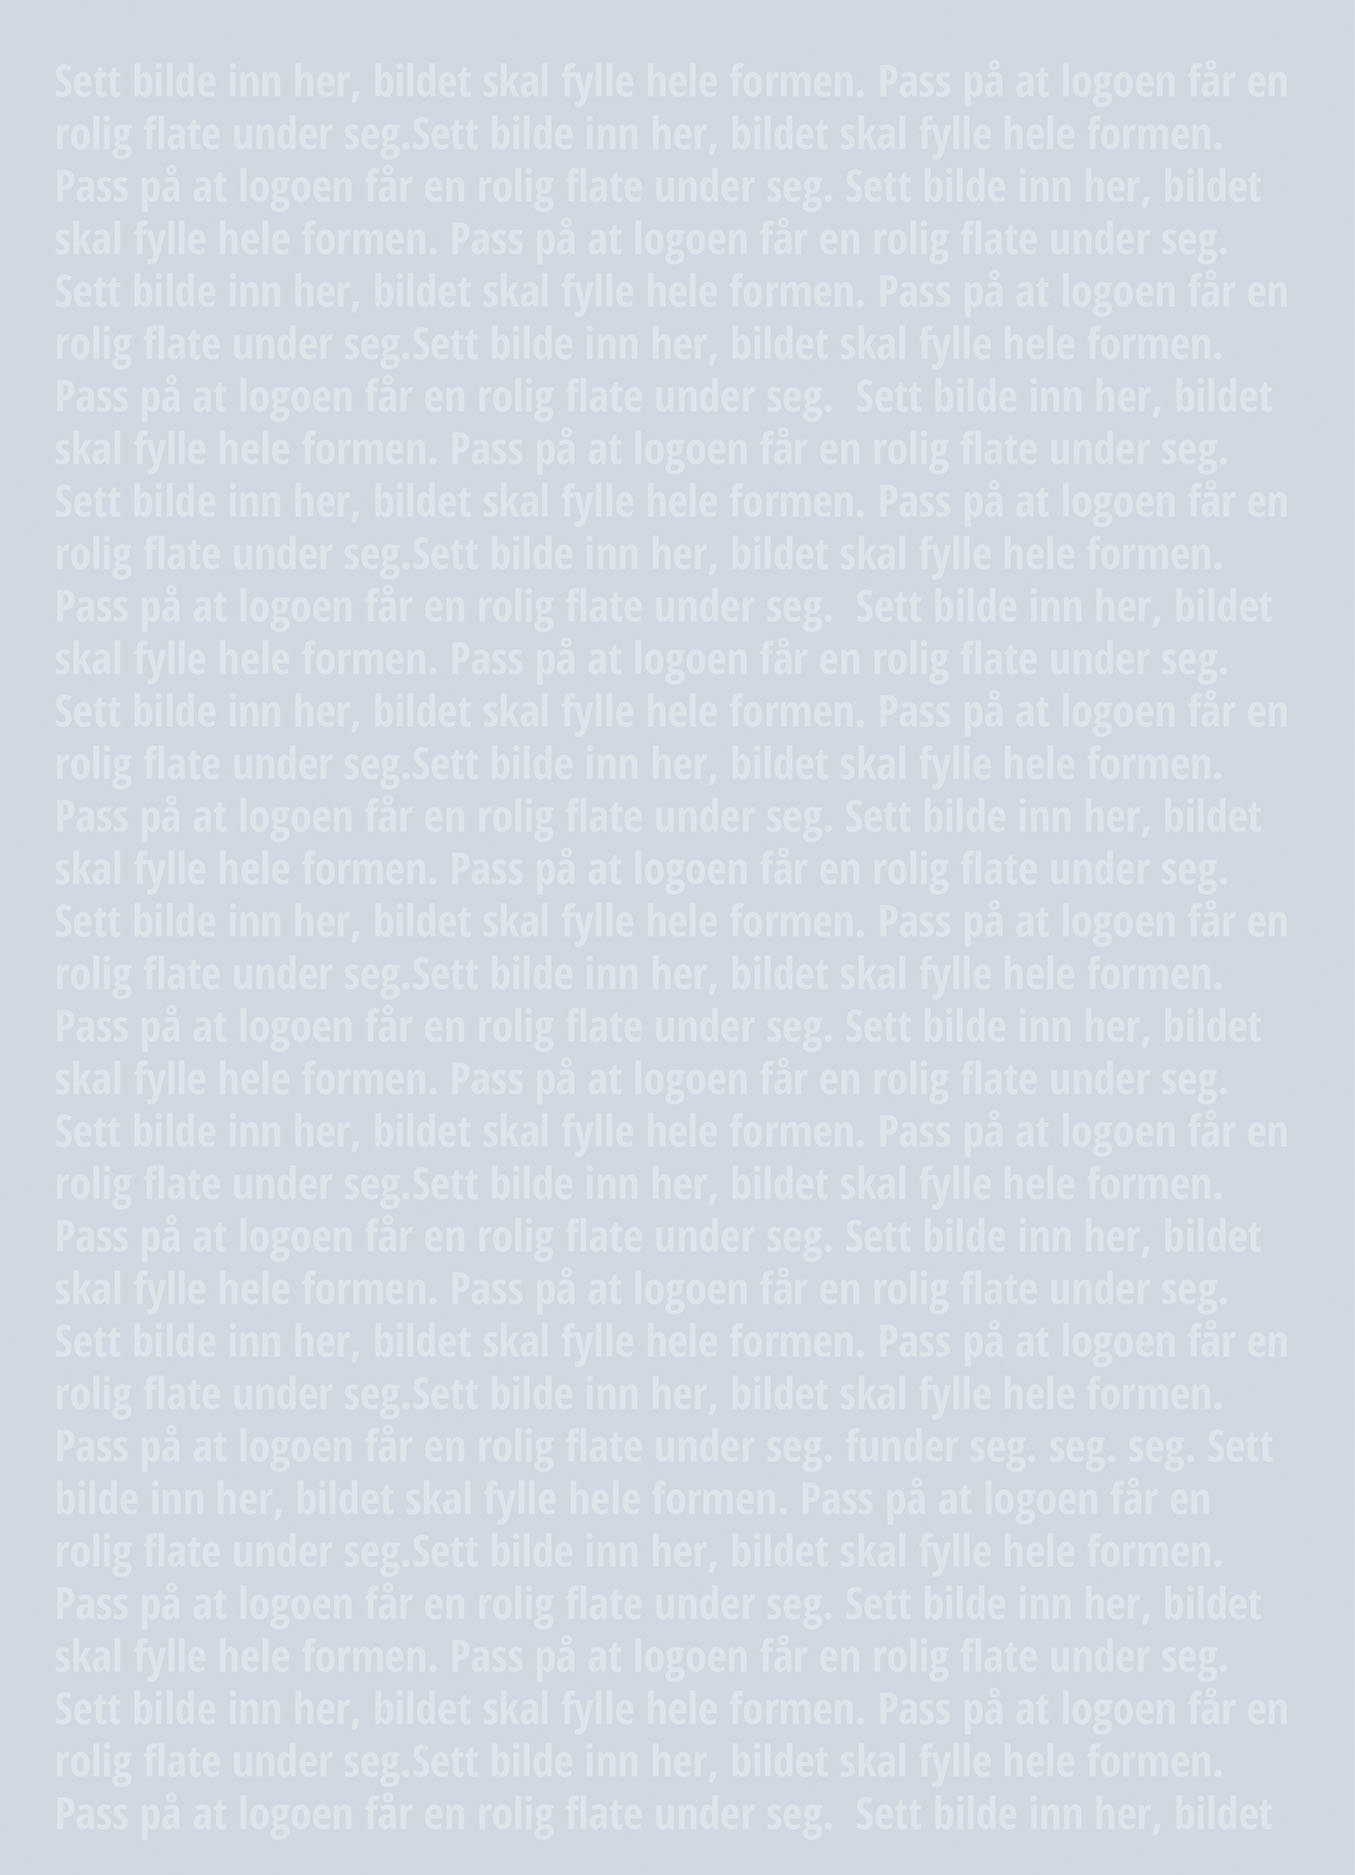
\includegraphics[scale=0.1]{example_image.jpg}
%\caption{Figure link should point to top of figure.}
%\label{fig:ex}
%\end{figure}


\chapter{Background and Related Work}
\begin{itemize}
\item Taking Sensor Networks from the Lab to the Jungle
\item Wireless Sensor Networks for Habitat Monitoring
\item Se de andre paperne Otto har sendt
\end{itemize}

\section{Something}
gggg

\chapter{Architecture}
Functionalities, abstractions, tell it clean/neat.

There are 6 components in the system: physical sensors, data storage, fused data, virtual sensors and the user. However, the main components in the system are the data storage, the fused data, the virtual sensors and the user.
In this chapter, we will describe the architecture of the data storage, fused data, virtual sensors and the user.The architecture of the system is presented in Figure \ref{fig:ex}.

\begin{figure}
\centering
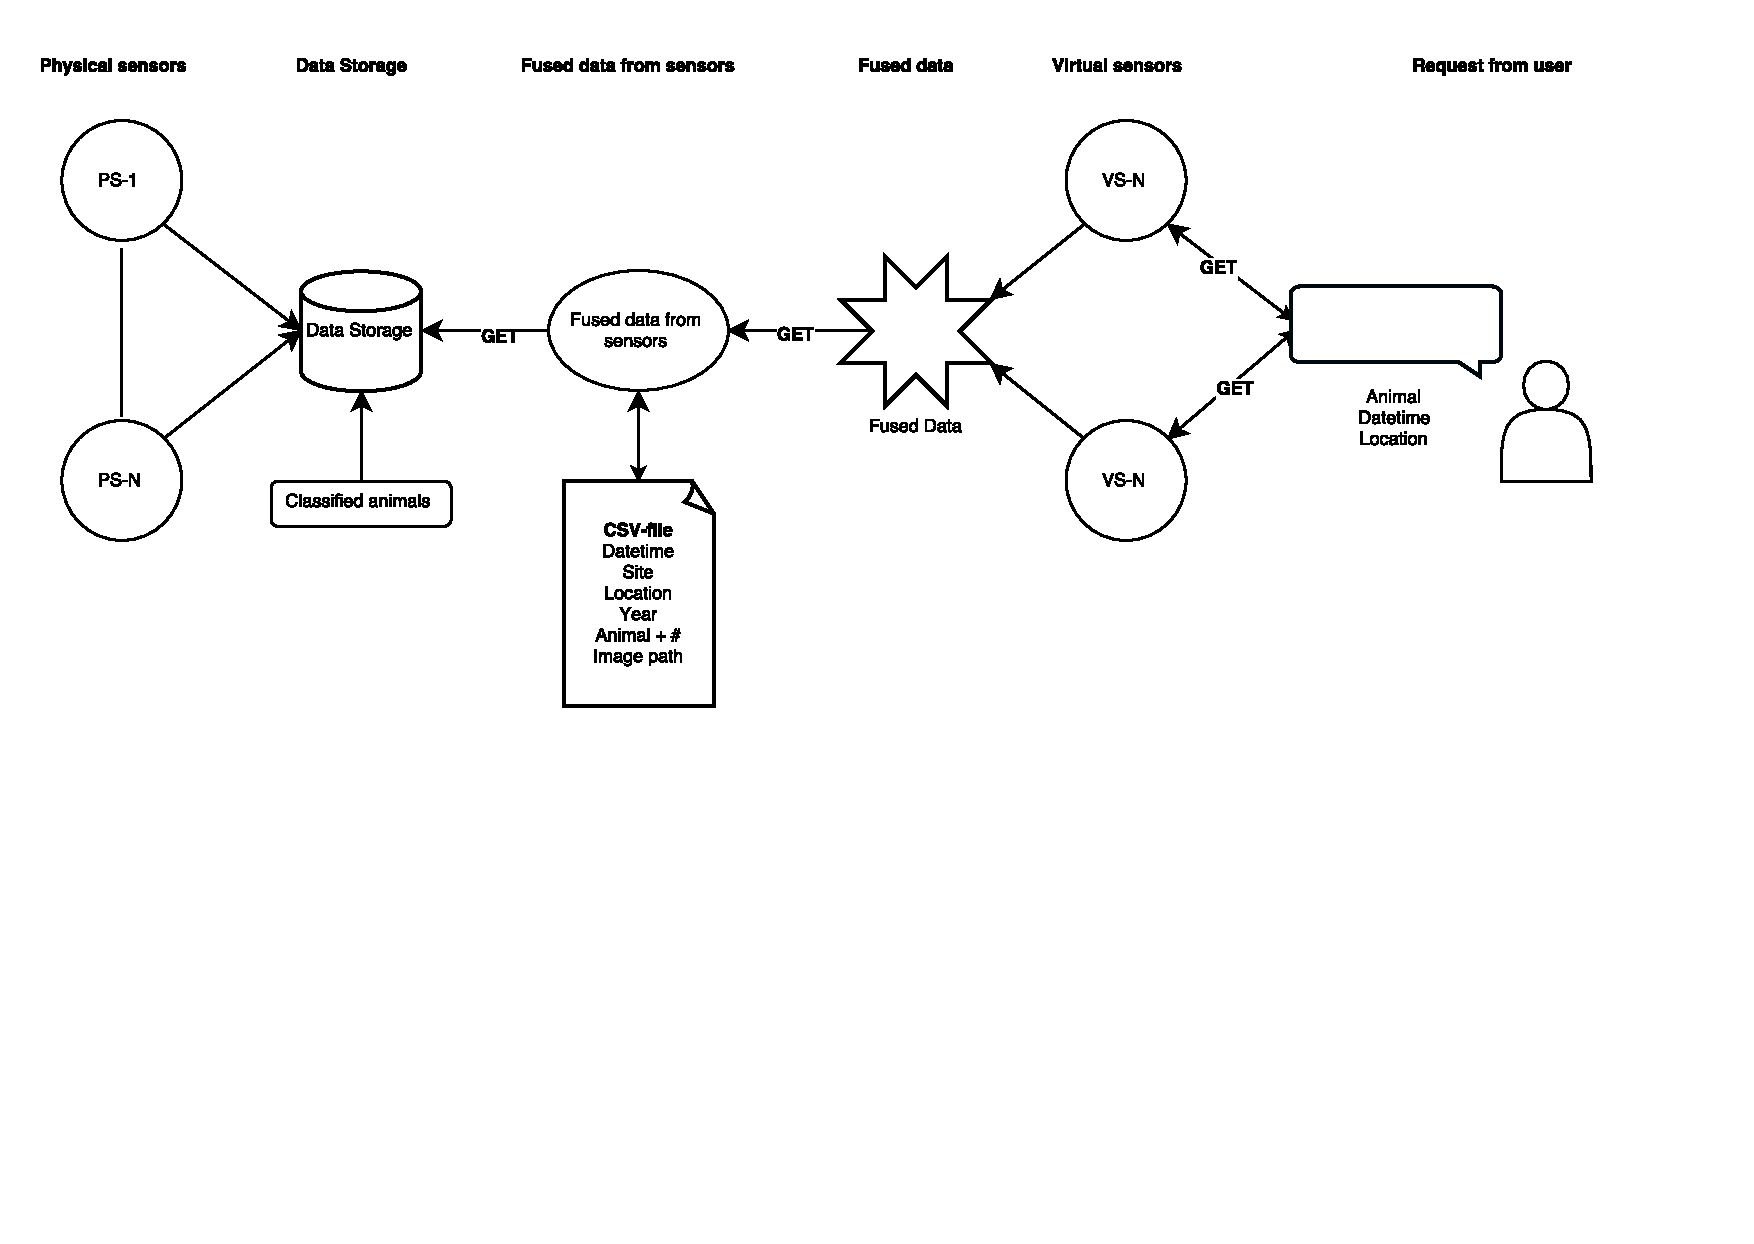
\includegraphics[scale=0.5]{Architecture.pdf}
\caption{Figure showing the system architecture.}
\label{fig:ex}
\end{figure}


\section{Physical Sensors and Data Storage}

The physical sensors transmit their data to the data storage. The data storage consists of (several set of) images from different sensors and excel-sheets containing information about each picture. 
The fused data retrieves it's data from the data storage and store the fused data into an CSV-file.

The virtual sensors are divided into animal-sensors, e.g. one raven-sensor, one red-fox- sensor etc.
The user types in what animal it wants to see, where it is and the date-time and the search is redirected to the sensor related to that specific animal. The virtual sensor receive its result from the fused data from the CSV-file.

Finally, the data/pictures is displayed to the user/biologist through a user interface(?)/image-shower (Python OpenCV library).


\section{Fused Data}
\section{Virtual Sensors}
\section{Result from Virtual Sensor to User}

\chapter{Design}
Client/Server, p2p, put/get, pub/sub, protokoller etc..
BESKRIV INTERAKSJONEN MELLOM ENHETENE!!

Virtual sensors probably uavhengige prosesser, ikke threads ettersom man evt vil addere flere sensorer og unnga a starte alle sensorer på nytt igjen..
Er de virtuelle sensorene servere eller publisher?

Rekursiv traversering av directories og leser metadata fra bildene (ca 1,6 mill bilder)) - Lagres i en dictionary hvor datetime og sted er key og image pathen er value).

Ca 16-17000 rows i et excel-ark. Leser ut info som dyr, antall, sted, datetime, site, year og putter i en string.

Disse sammenlignes og de som matcher blir skrevet til en CSV-fil.

\iffalse 
\begin{table}
\centering
\begin{tabular}{|l|l|}
\hline
Content left & Content right\\
\hline
\end{tabular}
\caption{A table}
\end{table}

%\begin{table}
%\centering
%\begin{tabular}{|l|l|}
%\hline
%Content left & Content right\\
%\hline
%\end{tabular}
%\caption{Another table}
%\end{table}


%\newpage

\begin{lstlisting}[frame=single,caption={Small C program},language=C]
#include "stdio.h"
#define e 3
#define g (e/e)
#define h ((g+e)/2)
#define f (e-g-h)
#define j (e*e-g)
#define k (j-h)
#define l(x) tab2[x]/h
#define m(n,a) ((n&(a))==(a))

long tab1[]={ 989L,5L,26L,0L,88319L,123L,0L,9367L };
int tab2[]={ 4,6,10,14,22,26,34,38,46,58,62,74,82,86 };

main(m1,s) char *s; {
  int a,b,c,d,o[k],n=(int)s;
  if(m1==1){ char b[2*j+f-g]; main(l(h+e)+h+e,b);
    printf(b); }
  else switch(m1-=h){
    case f:
      a=(b=(c=(d=g)<<g)<<g)<<g;
      return(m(n,a|c)|m(n,b)|m(n,a|d)|m(n,c|d));
    case h:
      for(a=f;a<j;++a)
        if(tab1[a]&&!(tab1[a]%((long)l(n))))
          return(a);
    case g:
      if(n<h)return(g);
      if(n<j){n-=g;c='D';o[f]=h;o[g]=f;}
      else{c='\r'-'\b';n-=j-g;o[f]=o[g]=g;}
      if((b=n)>=e)
        for(b=g<<g;b<n;++b)o[b]=o[b-h]+o[b-g]+c;
      return(o[b-g]%n+k-h);
    default:
      if(m1-=e) main(m1-g+e+h,s+g); else *(s+g)=f;
      for(*s=a=f;a<e;) *s=(*s<<e)|main(h+a++,
      (char *)m1);

    }
}
\end{lstlisting}

\fi

\chapter{Implementation}
%\lipsum[3-4]
Threads, data structures, language ...
Pandas (dataframe \footnote{\url{https://pandas.pydata.org/pandas-docs/stable/generated/pandas.DataFrame.html}} \footnote{\url{http://pandas.pydata.org/pandas-docs/stable/}}), CV2 (show image), exifread, Python 2.7, missing testing (CPU, memory, time?)


The system is implemented and written in Python 2.7\footnote{\url{https://www.python.org/}} because .. (frameworks available in this language??).

To visualize/show pictures, a Python library called OpenCV \footnote{\url{https://opencv-python-tutroals.readthedocs.io/en/latest/}} was implemented.
To read exif/metadata from pictures, we used a Python library called exifread 2.1.2 \footnote{\url{https://pypi.python.org/pypi/ExifRead}}.

\chapter{Evaluation} 
metrics, define (CPU, memoury, lantecy.), benchmarks (mirko, kernel...
How to measure, where done, PSEUDOCODE

\begin{itemize}
\item[Time] Finding folders and metadata takes:  1:43:13.488799,
Reading excel file takes:  0:00:17.413845,
Comparing takes:  4:43:30.705587,
Overall time is  6:27:01.608355.
Med alle bilder m/metadata og hele fotoboks2011_nordkynn_nordkynn.2011.xlsx.

\item[New time] Finding folders and metadata takes:  1:46:17.406581
Reading excel file takes:  0:01:07.686779
Comparing takes:  19:03:11.177869
Overall time is  20:50:36.271415
Med alle bilder m/mETADATA og hele nordkynn og varanger

This chapter describes the experimental setup and metrics used to evaluate the implemented system. 

\end{itemize}
\section{Experimental Setup}
All experiements was done on a Lenovo ThinkCenter with an Intel® Core™ i5-6400T CPU @ 2.20GHz × 4, Intel® HD Graphics 530 (Skylake GT2), 15,6 GiB memory and 503 GB disk. It ran on Ubuntu 17.04 64-bit.

\section{Something!?}
\section{Results}
What does the result say?
Each eksperiemnt, result, meaning

\chapter{Discussion}
Idea, architecture, design, results, andre løsninger, "arch har scaleproblem?"
\section{abcd}

\chapter{Contributions}

\chapter{Conclusion}
\section{Future Work}

\chapter{Future Work?}

\chapter{Appendix?}
readme, source code, dataset measurement RAW
\backmatter


%%% BIBLOGRAPHY

\newpage{}

\begin{thebibliography}{9}

\bibitem{coursebook}
 Robert Sedgewick 
  \emph{Algorithms in C - parts 1-4}.
  Addison-Wesley Publishing Company,
  3. Edition,
  1998.

\end{thebibliography}


\end{document}

